\section{AI Protocol and Capability Definition}

\subsection{Protocol Role}

The AI Protocol defines how capabilities are described. It specifies:
\begin{itemize}[leftmargin=*,nosep]
  \item \textbf{Providers:} entities offering AI or non-AI capabilities.
  \item \textbf{Models:} specific AI models with defined capabilities.
  \item \textbf{Capability Types:} categories of capabilities such as chat, embedding, and image generation.
  \item \textbf{Endpoints:} where capabilities can be invoked.
  \item \textbf{Parameters:} input and output schemas.
\end{itemize}

The protocol serves as the contract boundary between orchestration and execution: orchestration decides policy, while execution enforces invocation semantics.

The protocol is typically represented as structured manifests:
\begin{center}
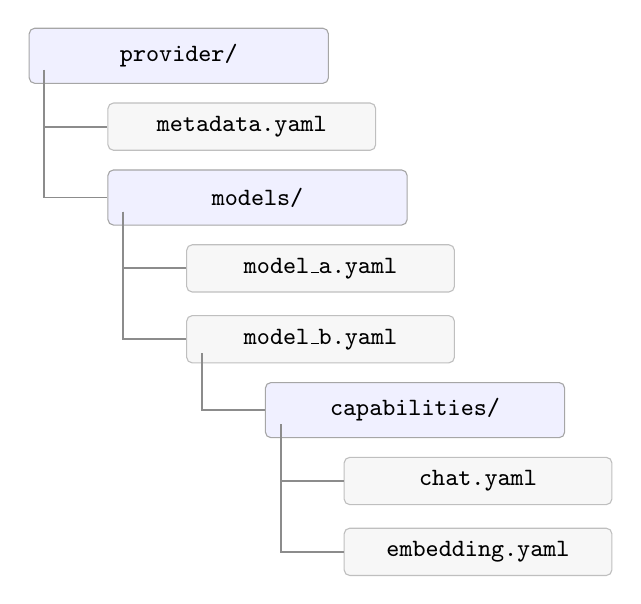
\begin{tikzpicture}[
  folder/.style={draw=black!35, rounded corners=2pt, fill=blue!6, minimum width=3.8cm, minimum height=0.7cm, align=left, font=\ttfamily\small, anchor=west},
  child/.style={draw=black!25, rounded corners=2pt, fill=gray!6, minimum width=3.4cm, minimum height=0.6cm, align=left, font=\ttfamily\small, anchor=west},
  line/.style={draw=black!45, line width=0.7pt}
]
\node[folder] (provider) at (0,0) {provider/};
\node[child] (metadata) at (1.0,-0.9) {metadata.yaml};
\node[folder] (models) at (1.0,-1.8) {models/};
\node[child] (modela) at (2.0,-2.7) {model\_a.yaml};
\node[child] (modelb) at (2.0,-3.6) {model\_b.yaml};
\node[folder] (caps) at (3.0,-4.5) {capabilities/};
\node[child] (chat) at (4.0,-5.4) {chat.yaml};
\node[child] (embed) at (4.0,-6.3) {embedding.yaml};

\draw[line] (provider.west) ++(0.2,-0.18) |- (metadata.west);
\draw[line] (provider.west) ++(0.2,-0.18) |- (models.west);
\draw[line] (models.west) ++(0.2,-0.18) |- (modela.west);
\draw[line] (models.west) ++(0.2,-0.18) |- (modelb.west);
\draw[line] (modelb.west) ++(0.2,-0.18) |- (caps.west);
\draw[line] (caps.west) ++(0.2,-0.18) |- (chat.west);
\draw[line] (caps.west) ++(0.2,-0.18) |- (embed.west);
\end{tikzpicture}
\end{center}

\subsection{Capability Definition}

Each capability is defined with:
\begin{itemize}[leftmargin=*,nosep]
  \item \textbf{Name:} a semantic identifier such as \texttt{generate\_text} or \texttt{search\_web}.
  \item \textbf{Input Schema:} a structured input specification.
  \item \textbf{Output Schema:} a structured output specification.
  \item \textbf{Execution Semantics:} the invocation and runtime behavior contract.
  \item \textbf{Quality Metadata ($Q$):} measured quality fields emitted by execution.
  \item \textbf{Pricing Metadata ($\Pi$):} metering and billing fields emitted by execution.
  \item \textbf{Provider Metadata:} information about the provider offering this capability.
\end{itemize}

\begin{quote}
\small
\begin{alltt}
name: generate\_text
description: Generate text based on a prompt
input\_schema:
  type: object
  properties:
    prompt:
      type: string
      description: The input prompt
    max\_tokens:
      type: integer
      description: Maximum tokens to generate
  required: [prompt]
output\_schema:
  type: object
  properties:
    text:
      type: string
      description: Generated text
execution:
  endpoint: /v1/completions
  method: POST
quality:
  telemetry\_fields: [execution\_latency\_ms, retry\_count]
pricing:
  billing\_model: per\_token
  currency: USD
provider:
  name: Example Provider
  version: 1.0.0
\end{alltt}
\end{quote}

\subsection{Provider-Centric Organization}

An important design decision is that capability descriptions remain provider-centric rather than capability-centric. The manifest structure follows:
\begin{center}
\texttt{Provider} $\rightarrow$ \texttt{Models} $\rightarrow$ \texttt{Capabilities}
\end{center}
rather than
\begin{center}
\texttt{Capability} $\rightarrow$ \texttt{Providers}.
\end{center}

The runtime can dynamically construct a capability index:
\begin{center}
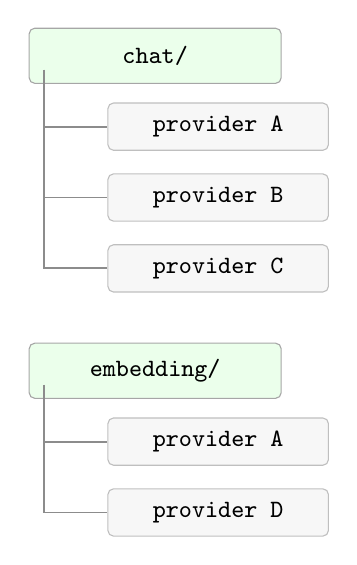
\begin{tikzpicture}[
  folder/.style={draw=black!35, rounded corners=2pt, fill=green!8, minimum width=3.2cm, minimum height=0.7cm, align=left, font=\ttfamily\small, anchor=west},
  child/.style={draw=black!25, rounded corners=2pt, fill=gray!6, minimum width=2.8cm, minimum height=0.6cm, align=left, font=\ttfamily\small, anchor=west},
  line/.style={draw=black!45, line width=0.7pt}
]
\node[folder] (chatf) at (0,0) {chat/};
\node[child] (pa) at (1.0,-0.9) {provider A};
\node[child] (pb) at (1.0,-1.8) {provider B};
\node[child] (pc) at (1.0,-2.7) {provider C};
\node[folder] (embedf) at (0,-4.0) {embedding/};
\node[child] (pea) at (1.0,-4.9) {provider A};
\node[child] (ped) at (1.0,-5.8) {provider D};

\draw[line] (chatf.west) ++(0.2,-0.18) |- (pa.west);
\draw[line] (chatf.west) ++(0.2,-0.18) |- (pb.west);
\draw[line] (chatf.west) ++(0.2,-0.18) |- (pc.west);
\draw[line] (embedf.west) ++(0.2,-0.18) |- (pea.west);
\draw[line] (embedf.west) ++(0.2,-0.18) |- (ped.west);
\end{tikzpicture}
\end{center}

This index can be rebuilt periodically and optimized based on user preferences, latency measurements, cost calculations, and reliability metrics.
